\documentclass[12pt,compress]{beamer}

\usetheme{ohnosequences}
\usecolortheme{ohnosequences}
\usefonttheme{ohnosequences}
\usepackage{amssymb}
% \usepackage{unicode-math}
\usepackage{fontspec,xltxtra,xunicode}

\let\OldHref\href
\renewcommand{\href}[2]{\OldHref[pdfnewwindow]{#1}{{\textbf{#2}}}}

\providecommand{\tightlist}{%
\setlength{\itemsep}{0pt}\setlength{\parskip}{0pt}}

% \setbeamertemplate{caption}[numbered]
% \setbeamertemplate{caption label separator}{:}
% \setbeamercolor{caption name}{fg=normal text.fg}
% \usepackage{amssymb,amsmath}
% \usepackage{ifxetex,ifluatex}
% \usepackage{fixltx2e} % provides \textsubscript
% \usepackage{lmodern}
%
% \usepackage{fontspec,xltxtra,xunicode}
% \defaultfontfeatures{Mapping=tex-text}
\newcommand{\euro}{€}

% use upquote if available, for straight quotes in verbatim environments
\IfFileExists{upquote.sty}{\usepackage{upquote}}{}
% use microtype if available
% \IfFileExists{microtype.sty}{\usepackage{microtype}}{}


% allow to break lines more easily on tt text
% http://tex.stackexchange.com/questions/52850/temporarily-increase-the-limit-on-space-size
\let\OldTexttt\texttt
\renewcommand{\texttt}[1]{ \emergencystretch=2em \OldTexttt{#1} }
% maybe?
\setlength{\emergencystretch}{3em}  % prevent overfull lines

\usepackage{graphicx}
\makeatletter
\def\maxwidth{\ifdim\Gin@nat@width>\linewidth\linewidth\else\Gin@nat@width\fi}
\def\maxheight{\ifdim\Gin@nat@height>\textheight0.8\textheight\else\Gin@nat@height\fi}
\makeatother
% Scale images if necessary, so that they will not overflow the page
% margins by default, and it is still possible to overwrite the defaults
% using explicit options in \includegraphics[width, height, ...]{}
\setkeys{Gin}{width=\maxwidth,height=\maxheight,keepaspectratio}
% no "Figure n" stuff
\usepackage{caption}
\captionsetup[figure]{labelformat=empty}
\setbeamertemplate{caption}{\insertcaption}

% Comment these out if you don't want a slide with just the
% part/section/subsection/subsubsection title:
% \AtBeginPart{
%   \let\insertpartnumber\relax
%   \let\partname\relax
%   \frame{\partpage}
% }
% \AtBeginSection{
%   \let\insertsectionnumber\relax
%   \let\sectionname\relax
%   \frame{\sectionpage}
% }
% \AtBeginSubsection{
%   \let\insertsubsectionnumber\relax
%   \let\subsectionname\relax
%   \frame{\subsectionpage}
% }

% \setlength{\parindent}{0pt}
% \setlength{\parskip}{6pt plus 2pt minus 1pt}
% \setlength{\emergencystretch}{3em}  % prevent overfull lines
% \providecommand{\tightlist}{%
%   \setlength{\itemsep}{0pt}\setlength{\parskip}{0pt}}
% % \setcounter{secnumdepth}{0}
% 
\hypersetup{
  setpagesize=false, % page size defined by xetex
  unicode=false, % unicode breaks when used with xetex
  xetex,
  pdfnewwindow,
  colorlinks,%
  citecolor=OldCyan-Dark,%
  filecolor=OldCyan-Dark,%
  linkcolor=OldCyan-Dark,%
  urlcolor=OldCyan-Dark,
  urlbordercolor=OldCyan-Dark
}



\usepackage{booktabs}
\usepackage[scale=2]{ccicons}

\title{Era7 bionformatics}
\subtitle{Presentación y Software Libre}
\author{Eduardo Pareja-Tobes, CTO}
\date{2016-05-06}

\institute{
  \href{http://era7bioinformatics.com}{{Era7} {\color{Grey-Light}bioinformatics}} - {\color{Salmon-Dark}oh}{\color{LightAmber-Dark}no}{\color{Grey}sequences}{\color{Salmon-Dark}!}
}

\begin{document}
\maketitle


% 
\section{Era7?}\label{era7}

\begin{frame}{Era7 bioinformatics}

\begin{block}{La empresa}

Fundada en \textbf{2006} en Granada, hacemos \textbf{análisis de datos}.
Genómica, principalmente de
\href{https://en.wikipedia.org/wiki/DNA_sequencing}{secuenciación de
ADN}.

\end{block}

\begin{block}{Claves}

\begin{itemize}
\tightlist
\item
  \textbf{Open source 100\%} \emph{Todo} lo que hacemos!
\item
  \textbf{Cloud computing} \emph{AWS}, cientos de servidores a diario
\item
  \textbf{Investigación} Bioinformática, Biología, Informática
\end{itemize}

\end{block}

\end{frame}

\begin{frame}{Equipo}

\begin{figure}[htbp]
\centering
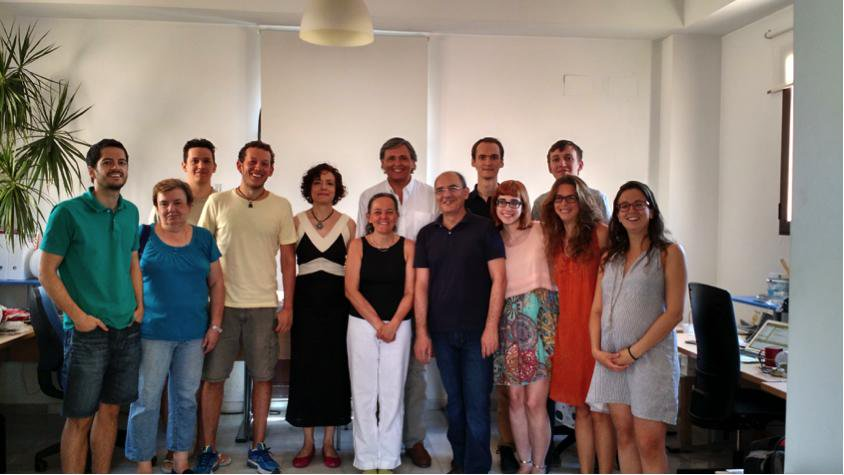
\includegraphics[width=0.80000\textwidth]{images/equipo.jpg}
\caption{\textbf{multidisciplinar}: Biólogos, Informáticos,
Matemáticos.}
\end{figure}

\end{frame}

\begin{frame}{Dónde?}

\begin{figure}[htbp]
\centering
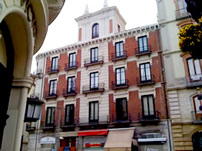
\includegraphics[width=0.60000\textwidth]{images/granada.jpg}
\caption{\textbf{Granada} En Puertal Real, el torreón encima del
Deutsche Bank.}
\end{figure}

\end{frame}

\begin{frame}{Dónde?}

\begin{figure}[htbp]
\centering
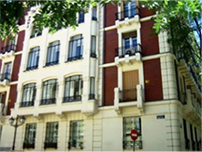
\includegraphics[width=0.60000\textwidth]{images/madrid.png}
\caption{\textbf{Madrid} al lado del Prado y del Ritz, somos gente con
clase.}
\end{figure}

\end{frame}

\begin{frame}{Dónde?}

\begin{figure}[htbp]
\centering
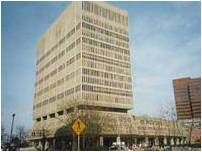
\includegraphics[width=0.60000\textwidth]{images/boston.jpg}
\caption{\textbf{Cambridge, MA}. Kendall square, enfrente del MIT. El
edificio \emph{todavía} no es entero nuestro.}
\end{figure}

\end{frame}

\begin{frame}{Clientes}

\begin{figure}[htbp]
\centering
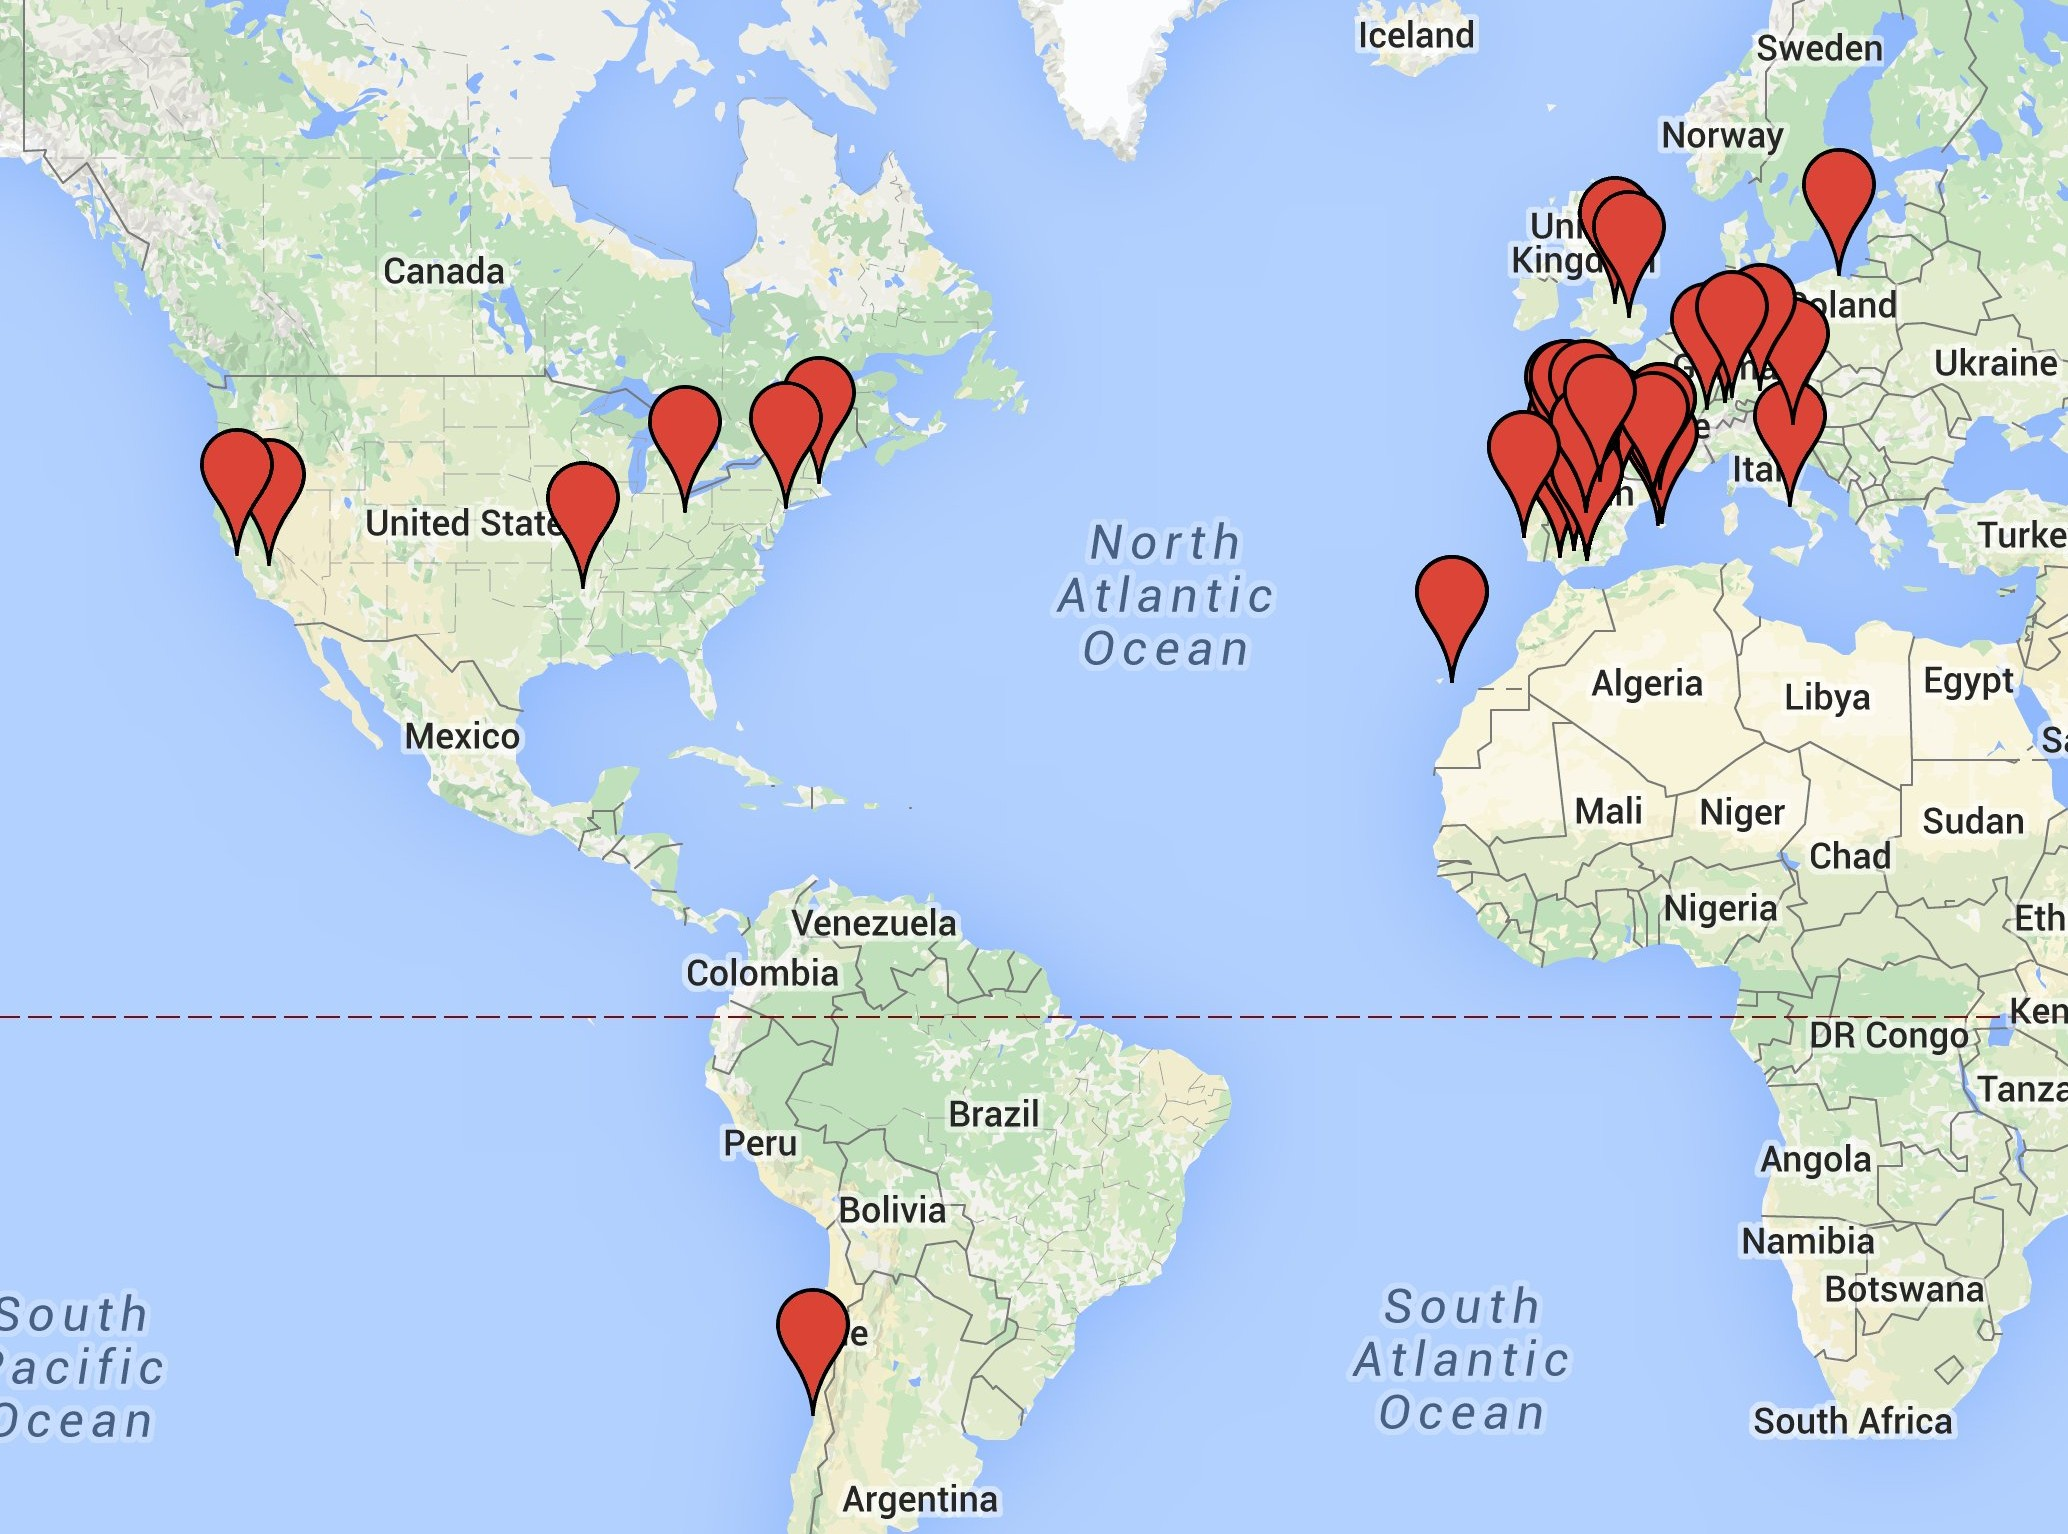
\includegraphics[width=0.70000\textwidth]{images/clients.jpg}
\caption{Centros de investigación, Empresas biotech, Hospitales,
\ldots{}}
\end{figure}

\end{frame}

\begin{frame}{Investigación}

~
\includegraphics[width=0.60000\textwidth]{images/ohnosequences.png}

~

Parte \textbf{fundamental} de nuestra actividad: en \textbf{2015} hemos
publicado \textbf{16} papers y preprints.

En \emph{qué?} \textbf{Bioinformática}, \textbf{Biología},
\textbf{Informática}: bacterial genomics, cloud data analysis, graph
databases, \ldots{}

\end{frame}

\section{Software libre!}\label{software-libre}

\begin{frame}{Nuestro modelo}

\textbf{Todo} lo que hacemos es \textbf{abierto}.

\emph{Licencia}?
\textbf{\href{https://tldrlegal.com/license/gnu-affero-general-public-license-v3-\%28agpl-3.0\%29}{AGPLv3}}.
100\% abierto, 100\%
\emph{\href{https://es.wikipedia.org/wiki/Copyleft}{copyleft}}.

Cobramos por hacer algo \emph{ahora} (servicios), no por lo que
\emph{hicimos} (licencias).

\end{frame}

\begin{frame}{Bio4j}

~
\includegraphics[width=0.40000\textwidth]{images/bio4j.png}

Plataforma para datos bioinformáticos/biológicos.

\begin{itemize}
\tightlist
\item
  Modelo basado en \textbf{typed graphs}
\item
  APIs genéricas en \textbf{Java} y \textbf{Scala} (unreleased)
\item
  \textbf{AWS} deployment
\end{itemize}

\end{frame}

\begin{frame}{GSoC14}

\begin{figure}[htbp]
\centering

\includegraphics{images/bio4jGsoc.png}
\caption{Seleccionados para el \emph{Google Summer of Code} de 2014.}
\end{figure}

\end{frame}

\begin{frame}{GitHub}

Desde \emph{2011}, para \textbf{todo}:

\begin{itemize}[<+->]
\tightlist
\item
  \textbf{Análisis de datos} primeros en coordinar \textbf{crowdsourced
  data analysis} en github:
  \href{https://github.com/ehec-outbreak-crowdsourced/BGI-data-analysis}{2011
  \emph{E. coli} outbreak}
\item
  \textbf{documentación} interna,
  \href{https://github.com/bio4j/bio4j.github.com}{websites},
  \href{https://github.com/ohnosequences/mg7/tree/master/docs/mg7-preprint}{papers},
  \href{https://github.com}{slides}
\item
  Y, por supuesto, \textbf{código!}
  \href{https://github.com/era7bio}{era7bio},
  \href{https://github.com/ohnosequences}{ohnosequences},
  \href{https://github.com/bio4j}{bio4j}
\end{itemize}

\end{frame}

\begin{frame}{Tecnologías, lenguajes, conocimiento}

No podríamos vivir sin \textbf{Amazon Web Services}, en particular
\emph{S3}, \emph{EC2}, \emph{SQS}, \emph{DynamoDB}.

\textbf{Graph databases} para Bio4j, para análisis de datos, \ldots{}

\emph{Lenguajes?} \textbf{Scala} en un 90\%, \textbf{Java} el resto.

Hay matemáticos sueltos, así que mucha \textbf{programación funcional} y
\textbf{teoría de categorías}.

\end{frame}

\begin{frame}{Qué estamos haciendo ahora}

\textbf{Muchos} proyectos interesantes! Dos ejemplos:

\pause

\begin{itemize}[<+->]
\tightlist
\item
  type-safe generic Scala \textbf{graph data APIs}, en desarrollo desde
  hace dos años
\item
  Diseño de un \textbf{graph database engine}
  (\href{http://www.idris-lang.org/}{\textbf{Idris}} + Scala)
\end{itemize}

\end{frame}

\begin{frame}{Conclusiones}

\pause

\begin{itemize}[<+->]
\tightlist
\item
  Es \textbf{posible} hacer todo \textbf{libre!}
\item
  Hay que currar \textbf{mucho}
\item
  Vale la pena
\end{itemize}

\end{frame}

\end{document}
